% The Why of Tali Forth
% Scot W. Stevenson

\begin{quote}
        Forth is well suited to resource-constrained situations. It doesn't need
        lots of memory and doesn't have much overhead. It can take full
        advantage of whatever hardware or interfaces exist.
\end{quote}
\begin{flushright}
        -- Charles Moore,\index{Moore, Charles} 
        \href{https://www.red-gate.com/simple-talk/opinion/geek-of-the-week/chuck-moore-geek-of-the-week/}{`Chuck
        Moore: Geek of the Week', redgate Hub 2009}
\end{flushright}

\section{The big picture}

This section provides background information on Forth, the 6502 processor, and
why anybody would want to combine the two. It can be safely skipped if you
already know all those things.

\subsection{The 6502 MPU}

It is a well-established fact that humanity reached the apex of processor design
with the 6502\index{6502} in 1976. Created by a team including Chuck
Peddle\index{Peddle, Chuck} and Bill Mensch\index{Mensch, Bill}, it was the
engine that powered the 8-bit home computer revolution of the
1980s.\footnote{Rumor has it that there was another MPU called `Z80'\index{Z80},
but it ended up being a mere footnote.} The VIC-20\index{VIC-20}, Commodore
PET\index{Commodore PET}, Apple II\index{Apple II}, and Atari 800\index{Atari
800} all used the 6502, among others. 

\begin{figure}[h !]
        \centering
        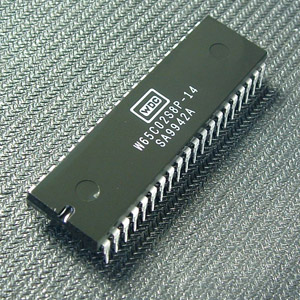
\includegraphics[width=0.5\textwidth]{pics/W65c02}
        \caption{\textit{The 65c02 MPU.} Photo: Anthony King, released in 
        the public domain}
        \label{fig:65c02}
\end{figure}

More than 40 years later, the processor is still in production by the \href
{http://www.westerndesigncenter.com/wdc/w65c02s-chip.cfm}{Western Design
Center}\index{WDC}. Apart from commercial uses, there is an active hobbyist
scene centered on the website \href{http://6502.org/}{6502.org}.\index{6502.org}
Quite a number of people have built their own 8-bit computers based on this chip
and the instructions there, including a
\href{http://wilsonminesco.com/6502primer/}{a primer} by Garth
Wilson\index{Wilson, Garth}. It is for these systems that Tali Forth 2 was
created.

The most important variant of the 65c02 produced today is the \href
{https://en.wikipedia.org/wiki/WDC\_65C02}{65c02}\index{65c02}, a CMOS chip with
some additional instructions. It is for this chip that Tali Forth 2 was written. 

But why program in 8-bit assembler at all?\footnote{Wilson\index{Wilson,
Garth} answers this question in greater detail as part of his
\href{http://wilsonminesco.com/6502primer/65tutor\_intro.html}{6502 primer}} The
65c02 is fun to work with because of its clean instruction set architecture
(ISA)\index{instruction set!architecture}\index{ISA|see {instruction set}}. This
is not the place to explain the joys of assembler. The official handbook for the
65c02 is \textit{Programming the 65816, including the 6502, 65C02 and
65802}\cite{eyeslichty}.


\subsection{Forth}

\begin{quote}
        If C gives you enough rope to hang yourself, Forth is a flamethrower
        crawling with cobras.
\end{quote}
\begin{flushright}
        -- Elliot Williams,\index{Williams, Elliot} \href{https://hackaday.com/2017/01/27/forth-the-hackers-language/}{
        \textit{Forth: The Hacker's Language}}
\end{flushright}

Forth\index{Forth|textbf} is the \textit{enfant terrible} of programming
languages. It was invented by Charles `Chuck' Moore\index{Moore, Charles} in the
1960s to do work with radio astronomy, way before there were modern operating
systems or programming languages.\footnote{A brief history of Forth can be found
at \href{https://www.forth.com/resources/forth-programming-language/}
{https://www.forth.com/resources/forth-programming-language/}} As a language for
people who actually need to get things done, it lets you run with scissors, play
with fire, and cut corners until you've turned a square into a circle. Forth is
not for the faint-hearted: It is trivial, for instance, to redefine 1 as 2 and
\texttt{true}\index{true@\texttt{true}} as
\texttt{false}.\index{false@\texttt{false}} Though you can do really, really
clever things with few lines of code, the result can be hard for other people to
understand, leading to the reputation of Forth begin a `write-only language'.
However, Forth excels when you positively, absolutely have to get something done
with hardware that is really too weak for the job. 

It should be no surprise that NASA\index{NASA} is one of the organizations who
use Forth. The \textit{Cassini} mission\index{Cassini@\textit{Cassini}} to
Saturn used a
\href{http://www.cpushack.com/2013/02/21/charles-moore-forth-stack-processors/}{Forth
CPU}, for instance. It is also perfect for small computers like the 8-bit 65c02.
After a small boom in the 1980s, more powerful computers led to a decline of the
language. The `Internet of Things' with embedded small processors has led to a
certain amount
\href{https://www.embedded.com/design/programming-languages-and-tools/4431133/Go-Forth-}{renewed
interest} in the language. It helps that Forth is easy to implement: It is
stack-based, uses reverse polish notation (RPN)\index{RPN|see {reverse polish
notation}}\index{reverse polish notation} and a simple threaded\index{threading}
interpreter model. 

There is no way this document can provide an adiquate introduction to Forth.
There are quite a number of tutorials, however, such as \textit{A Beginner's
Guide to Forth} by J.V.~Nobel\cite{nobel} or the classic (but slightly dated)
\textit{Starting Forth}\cite{brodie03} by Leo Brodie\index{Brodie, Leo}.
Gforth,\index{Gforth} one of the more powerful free Forths, comes with its own
\href{http://www.complang.tuwien.ac.at/forth/gforth/Docs-html/Tutorial.html}{tutorial}.\footnote{Once
you have understood the basics of the language, do yourself a favor and read
\textit{Thinking Forth} by Brodie\cite{brodie84}\index{Brodie, Leo}, which deals
with the philosophy of the language. Like Lisp\index{Lisp}, exposure to Forth
will change the way you think about programming.} 


\section{Writing your own Forth}

Even if the 65c02 is great and Forth is brilliant, why got to the effort of
writing a new, bare-metal version of the languages? After almost 50 years,
shouldn't there be a bunch of Forths around already?


\subsection{FIG Forth}

In fact, the classic Forth availble for the whole group of 8-bit MPUs is FIG
Forth\index{FIG Forth} -- `FIG' stands for `Forth Interest Group'. Ported to
various architectures, it was original based on an incarnation for the 6502
written by Bill Ragsdale\index{Ragsdale, Bill} and Robert Selzer\index{Selzer,
Robert}. There are PDFs of the
\href{http://www.forth.org/fig-forth/fig-forth\_6502.pdf}{6502 version} from
September 1980 freely available -- Forths are traditionally placed in the public
domain -- and more than one hobbyist has revised it to his machine. 

However, Forth has changed a lot in the past three decades. There is now a
standardized version called \href{https://forth-standard.org/}{ANSI Forth
standard}\index{ANSI Forth}, which includes such basic changes as how the
\texttt{do} loop works. Learning the language with FIG Forth is like learning
English with \textit{The Canterbury Tales}.\index{Canterbury Tales,
The@\textit{Canterbury Tales, The}}


\subsection{A modern Forth for the 65c02}

Tali Forth was created to provide an easy to understand modern Forth written
especially for the 65c02 that anybody can understand, adapt to their own use,
and maybe actually work with. As part of that effort, the source code is heavily
commented. And this document tries to explain the internals in more detail.

% end
